\chapter{De la conservación local a las ecuaciones de campo de Einstein}

Las ecuaciones de campo de Einstein son lo bastante sencillas como para escribirse en una sola línea, pero notoriamente engorrosas al desarrollarlas por componentes. Una métrica tiene muchos símbolos de Christoffel; estos contienen derivadas de la métrica, y el tensor de curvatura contiene tanto derivadas como productos de símbolos de Christoffel. Incluso antes de intentar resolver nada, el cálculo puede ocupar páginas. Para una métrica concreta, el software simbólico suele ser una forma sensata de manejar ese cúmulo de operaciones.

Los principios son mucho más claros que el cálculo. Por eso no empezaremos atacando las ecuaciones componente por componente. Nos preguntaremos qué tipo de ecuación exige la gravedad. El argumento parte de la teoría de Newton, pasa por la conservación local y termina al hallar la única combinación de tensores de curvatura que puede igualarse coherentemente al flujo y la densidad de energía y momento. A lo largo del capítulo usamos \(c=1\).

\section{La doble dirección de la teoría de Newton}

La gravedad encierra dos instrucciones complementarias. El campo gravitatorio indica a la materia cómo moverse, mientras que la materia indica al campo gravitatorio qué debe ser. Esta doble dirección ya se aprecia en la mecánica newtoniana.

Sea \(\phi(\mathbf{x},t)\) el potencial gravitatorio newtoniano. Un cuerpo de prueba de masa \(m\) experimenta la fuerza
\begin{equation}
 \mathbf{F}=-m\nabla\phi.
\end{equation}
Al combinar esto con \(\mathbf{F}=m\mathbf{a}\), la masa de prueba se cancela:
\begin{equation}
 \mathbf{a}=-\nabla\phi.
\end{equation}
Esta es la primera dirección de la relación. Una vez conocido el campo, este indica cómo acelera todo cuerpo en caída libre, con independencia de su masa.

La dirección inversa viene dada por la ecuación de Poisson,
\begin{equation}
 \nabla^2\phi=4\pi G\rho,
 \qquad
 \nabla^2=
 \frac{\partial^2}{\partial x^2}
 +\frac{\partial^2}{\partial y^2}
 +\frac{\partial^2}{\partial z^2},
 \label{eq:poisson}
\end{equation}
donde \(\rho(\mathbf{x},t)\) es la masa por unidad de volumen. El factor \(4\pi\) podría incorporarse a la definición de \(G\), pero solo reaparecería en otro lugar. La ecuación~\eqref{eq:poisson} indica que la distribución de materia es la fuente del potencial.

Para un cuerpo esféricamente simétrico de masa total \(M\), la solución exterior es
\begin{equation}
 \phi(r)=-\frac{GM}{r}.
 \label{eq:newton-potential}
\end{equation}
La densidad puede estar concentrada cerca del centro, distribuida uniformemente o disminuir gradualmente hacia la superficie. La solución exterior solo depende de la simetría esférica y de la masa total. Fuera de la materia,
\(\nabla^2\phi=0\); al derivar \(1/r\) se obtiene entonces la fuerza inversamente proporcional al cuadrado de la distancia. Si solo nos interesa el exterior, podemos reducir la fuente a un punto y usar la misma expresión en todas partes salvo en ese punto.

\begin{classroomqa}
\audiencequestion{¿Debe ser constante la densidad dentro del cuerpo esférico y luego saltar discontinuamente a cero en su límite?}
\lecturerresponse{No. Para este argumento debe tener simetría esférica, pero no tiene por qué ser constante ni presentar un salto. Puede disminuir suavemente hasta cero. Ninguno de esos detalles del interior cambia el potencial exterior, que depende únicamente de la masa total.
\lecturetimestamp{00:09:13--00:09:37}}
\end{classroomqa}

Esta formulación en términos de campo parece más local que una fuerza directa entre masas distantes, pero la gravedad newtoniana sigue implicando acción instantánea a distancia. Si se mueve la fuente, el potencial newtoniano cambia de inmediato en todas partes. La relatividad general debe sustituir tanto esa respuesta instantánea como la ley de fuerza.

\section{Una pista del campo débil, todavía no una ecuación}

La versión relativista de la primera instrucción ya se conoce: dada la métrica del espacio-tiempo, las partículas en caída libre siguen geodésicas del espacio-tiempo. Ahora necesitamos la sustitución relativista de la ecuación de Poisson: la instrucción que establece cómo determina la materia la métrica.

La geometría de Schwarzschild ofrece una pista. Su componente temporal-temporal es
\begin{equation}
 g_{00}=1-\frac{2GM}{r}.
\end{equation}
Al usar la ecuación~\eqref{eq:newton-potential}, queda
\begin{equation}
 g_{00}=1+2\phi.
\end{equation}
Por consiguiente,
\begin{equation}
 \nabla^2g_{00}=2\nabla^2\phi=8\pi G\rho.
 \label{eq:weak-mnemonic}
\end{equation}

La ecuación~\eqref{eq:weak-mnemonic} debe tomarse con cautela. Es un recurso mnemotécnico, no la ecuación de Einstein. Utiliza una componente preferida de la métrica y una fuente no relativista. Aun así, muestra la estructura que buscamos: una densidad de materia en un lado y derivadas segundas de la geometría en el otro. Es el puente aproximado entre la ecuación de Poisson y una ecuación de campo covariante.

Ahora hay que examinar con más atención el lado derecho. En unidades relativistas, la masa es energía, así que \(\rho\) debe entenderse primero como una densidad de energía. Pero una densidad de energía no es un objeto relativista completo. Para ver qué la acompaña, empezaremos por una cantidad conservada más sencilla.

\section{Densidad de carga, corriente y conservación local}

Sea \(Q\) la carga eléctrica y denote \(\sigma\) la densidad de carga:
\begin{equation}
 \sigma=\lim_{\Delta V\to0}\frac{\Delta Q}{\Delta V}.
\end{equation}
La densidad indica cuánta carga ocupa un pequeño volumen espacial en un instante. La corriente plantea otra pregunta. Coloquemos en el espacio una ventana infinitesimal orientada y contemos cuánta carga la atraviesa por unidad de área y por unidad de tiempo. Las tres orientaciones posibles dan las componentes espaciales de la corriente \(J^i\).

La comparación dimensional es instructiva. La densidad de carga es la carga dividida por tres longitudes espaciales. La corriente es la carga dividida por dos longitudes espaciales y un intervalo de tiempo. Cuando \(c=1\), el tiempo y la longitud tienen las mismas unidades, de modo que la densidad y la corriente tienen dimensiones compatibles. Se combinan en un cuadrivector:
\begin{equation}
 J^\mu=(J^0,J^1,J^2,J^3),
 \qquad J^0=\sigma.
\end{equation}

La conservación de la carga no se limita a afirmar que la carga total del universo permanece constante. Es local. La carga no puede desaparecer del aula y reaparecer instantáneamente en Alfa Centauri. Si sale de una región, debe atravesar su frontera. En una caja pequeña, la disminución de la carga en su interior es igual al flujo saliente a través de sus paredes. El teorema de Gauss da
\begin{equation}
 \dot{\sigma}+\nabla\cdot\mathbf{J}=0,
\end{equation}
o, usando la convención de suma,
\begin{equation}
 \partial_\mu J^\mu=0.
 \label{eq:charge-continuity}
\end{equation}
En coordenadas curvas, la ecuación tensorial correspondiente se escribe con una derivada covariante:
\begin{equation}
 D_\mu J^\mu=0.
\end{equation}
La derivada covariante no es un adorno. Hace que el enunciado tenga sentido en cualquier sistema de coordenadas.

\section{Por qué la energía y el momento requieren dos índices}

La carga en sí es invariante. Observadores en movimiento relativo coinciden en la carga de un electrón, aunque no en la densidad de carga ni en la corriente. Un observador en movimiento ve volúmenes contraídos por Lorentz y puede observar un flujo de cargas donde otro observa cargas en reposo. Por tanto, la densidad y la corriente se mezclan al cambiar de sistema de referencia, aunque la carga total no lo haga.

La energía y el momento son más complicados. Incluso sus valores totales dependen del sistema de referencia. Un observador puede ver una partícula en reposo, con solo su energía en reposo y sin momento espacial. Otro observador que pasa junto a ella ve tanto energía cinética como momento. Las cuatro cantidades forman el cuadrivector de momento
\begin{equation}
 P^\nu=(P^0,P^1,P^2,P^3),
 \qquad P^0=E.
\end{equation}
Cada componente \(P^\nu\) se conserva localmente. Por tanto, cada una tiene una densidad y un flujo. Un índice identifica la cantidad conservada; el otro, si se trata de una densidad o de una dirección de flujo.

Empecemos por la energía. Su densidad es \(T^{00}\). La energía también puede atravesar una ventana, así que \(T^{0i}\) es el flujo de energía en la dirección \(x^i\). Consideremos ahora la componente \(i\) del momento. Su densidad es \(T^{i0}\), y su flujo en la dirección \(x^j\) es \(T^{ij}\). Con esta convención:
\begin{itemize}
 \item \(T^{00}\) es la densidad de energía;
 \item \(T^{0i}\) es el flujo de energía en la dirección \(i\);
 \item \(T^{i0}\) es la densidad de la componente \(i\) del momento;
 \item \(T^{ij}\) es el flujo de momento \(i\) a través de una superficie cuya normal apunta en la dirección \(j\).
\end{itemize}
Más adelante reconoceremos que el bloque espacial \(T^{ij}\) representa los esfuerzos: sus elementos diagonales incluyen las presiones, mientras que los elementos no diagonales describen el esfuerzo cortante.

\begin{classroomqa}
\audiencequestion{Cuando \(T^{m0}(x)\) se llama densidad de la componente \(m\) del momento, ¿\(x\) significa la componente \(m\) de la posición?}
\lecturerresponse{No. El argumento \(x\) denota la posición en el espacio-tiempo donde se evalúa la densidad; representa todas las coordenadas. El índice \(m\) señala qué componente del momento se cuenta.
\lecturetimestamp{00:41:07--00:41:27}}
\end{classroomqa}

Para cada \(\nu\) fijo, la conservación local da una ecuación de continuidad:
\begin{equation}
 D_\mu T^{\nu\mu}=0.
 \label{eq:stress-continuity}
\end{equation}
Los cuatro valores de \(\nu\) dan una ecuación para la energía y tres para el momento. En conjunto, las densidades y los flujos forman el tensor de energía-momento.

\begin{figure}[htbp]
\centering
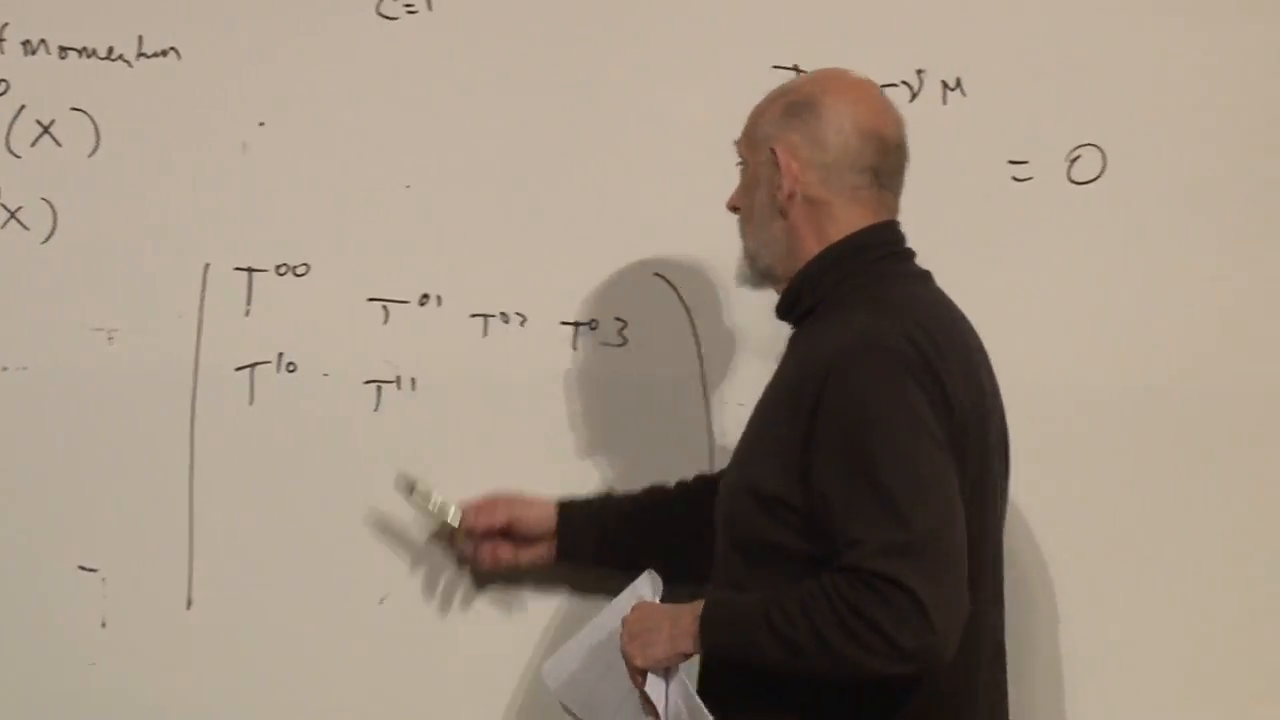
\includegraphics[width=0.84\textwidth]{lecture_09_figure_02.png}
\caption{El tensor de energía-momento que se va construyendo en la pizarra. El primer índice selecciona la energía o una componente del momento; el segundo, la densidad o el flujo.}
\lectureframe{00:44:30}
\end{figure}

La matriz completa es
\begin{equation}
 T^{\mu\nu}=
 \begin{pmatrix}
 T^{00}&T^{01}&T^{02}&T^{03}\\
 T^{10}&T^{11}&T^{12}&T^{13}\\
 T^{20}&T^{21}&T^{22}&T^{23}\\
 T^{30}&T^{31}&T^{32}&T^{33}
 \end{pmatrix}.
\end{equation}
Un teorema adicional de la mecánica relativista y la teoría de campos establece que el tensor de energía-momento relevante para la gravedad es simétrico:
\begin{equation}
 T^{\mu\nu}=T^{\nu\mu}.
 \label{eq:stress-symmetry}
\end{equation}
En particular, el flujo de energía y la densidad de momento son los elementos no diagonales correspondientes, vistos desde lados opuestos. La simetría también permite escribir la ecuación~\eqref{eq:stress-continuity} en la forma habitual
\begin{equation}
 D_\mu T^{\mu\nu}=0.
 \label{eq:stress-conservation}
\end{equation}

\begin{classroomqa}
\audiencequestion{¿Por qué el tensor de energía-momento tiene un índice adicional, mientras que la corriente de carga solo necesita uno?}
\lecturerresponse{El índice de la corriente ya distingue la densidad de la dirección del flujo. La carga no necesita una etiqueta adicional porque la carga conservada es un escalar. La energía y las tres componentes del momento son, en sí mismas, cuatro componentes, así que el primer índice indica de qué cantidad conservada se trata y el segundo señala si es una densidad o un flujo.
\lecturetimestamp{00:45:31--00:47:24}}
\end{classroomqa}

\begin{classroomqa}
\audiencequestion{¿Es simétrica toda la matriz \(T^{\mu\nu}\), y no solo los elementos de flujo de energía y densidad de momento?}
\lecturerresponse{Sí. Toda la matriz es simétrica. Más adelante se explicará en detalle el significado de sus elementos espaciales, incluidas la presión y los esfuerzos.
\lecturetimestamp{00:47:32--00:47:54}}
\end{classroomqa}

Así pues, la densidad de energía era solo una parte de un objeto más amplio. La fuente de la gravedad no puede ser coherentemente solo \(T^{00}\); debe involucrar el tensor completo.

\section{Una ley no puede seleccionar una sola componente}

La necesidad de una ecuación tensorial se aprecia sin calcular ninguna curvatura. Supongamos que \(A_i\) y \(B_i\) son vectores y que una ley propuesta solo afirma \(A_3=B_3\). Si esa igualdad debe cumplirse en todo sistema de referencia girado, giremos el tercer eje hasta alinearlo con el segundo. La misma ley afirmará entonces \(A_2=B_2\); otro giro da \(A_1=B_1\). En realidad, la ley independiente del sistema de referencia era la ecuación vectorial
\begin{equation}
 A_i=B_i.
\end{equation}

Las transformaciones de Lorentz extienden el mismo argumento al tiempo. Si \(A^0=B^0\) debe cumplirse en todos los sistemas inerciales, los cambios de sistema mediante impulsos de Lorentz mezclan la componente temporal con las espaciales y exigen la ecuación completa \(A^\mu=B^\mu\). Las leyes relativistas correctas deben igualar tensores del mismo tipo.

El recurso mnemotécnico newtoniano destacaba \(T^{00}\), pero la ecuación relativista debe tener la forma
\begin{equation}
 G_{\mu\nu}=8\pi G\,T_{\mu\nu},
 \label{eq:field-schematic}
\end{equation}
donde el símbolo \(G_{\mu\nu}\) es, por ahora, solo un marcador provisional. Sus propiedades necesarias ya están claras:
\begin{enumerate}
 \item debe ser un tensor simétrico de rango dos;
 \item debe construirse a partir de la métrica, no de la materia;
 \item debe contener dos derivadas de la métrica;
 \item su divergencia covariante debe anularse.
\end{enumerate}
La última condición se desprende de la ecuación~\eqref{eq:stress-conservation}.

\section{La búsqueda entre los tensores de curvatura}

Los símbolos de Christoffel contienen una derivada de la métrica:
\begin{equation}
 \Gamma^\sigma_{\tau\nu}
 =
 \frac12 g^{\sigma\delta}
 \left(
 \partial_\tau g_{\delta\nu}
 +\partial_\nu g_{\delta\tau}
 -\partial_\delta g_{\tau\nu}
 \right).
 \label{eq:christoffel}
\end{equation}
No son tensores, así que no pueden proporcionar por sí mismos el lado izquierdo. El tensor de curvatura de Riemann sí es un tensor:
\begin{equation}
 R^\rho{}_{\sigma\mu\nu}
 =
 \partial_\mu\Gamma^\rho_{\nu\sigma}
 -\partial_\nu\Gamma^\rho_{\mu\sigma}
 +\Gamma^\rho_{\mu\lambda}\Gamma^\lambda_{\nu\sigma}
 -\Gamma^\rho_{\nu\lambda}\Gamma^\lambda_{\mu\sigma}.
 \label{eq:riemann}
\end{equation}
Sus dos primeros términos contienen derivadas segundas de la métrica; los dos últimos contienen productos de primeras derivadas. Este es justamente el orden diferencial que sugiere la ecuación newtoniana.

El problema está en la estructura de índices. \(R^\rho{}_{\sigma\mu\nu}\) tiene cuatro índices, mientras que \(T_{\mu\nu}\) tiene dos. Al contraer un índice superior adecuado con uno inferior se obtiene el tensor de Ricci,
\begin{equation}
 R_{\mu\nu}=R^\lambda{}_{\mu\lambda\nu}.
 \label{eq:ricci}
\end{equation}
Otras contracciones aparentes se anulan por las simetrías del tensor de Riemann o reproducen el mismo objeto, salvo por un signo y la convención de índices. El tensor de Ricci es simétrico, pero contiene menos información que el tensor de Riemann completo: puede anularse mientras el tensor de Riemann sigue siendo distinto de cero.

\begin{classroomqa}
\audiencequestion{¿Se pueden contraer sin más dos índices inferiores del tensor de Riemann? ¿No exige una contracción un índice covariante y otro contravariante?}
\lecturerresponse{Exactamente. Primero hay que elevar un índice con la métrica inversa o, de forma equivalente, incluir \(g^{\mu\nu}\) en la contracción. Escrita como \(R^\lambda{}_{\mu\lambda\nu}\), queda explícito el par de índices superior e inferior requerido.
\lecturetimestamp{01:00:09--01:00:33}}
\end{classroomqa}

Al contraer de nuevo el tensor de Ricci se obtiene el escalar de curvatura,
\begin{equation}
 R=g^{\mu\nu}R_{\mu\nu}.
 \label{eq:ricci-scalar}
\end{equation}
Al multiplicar este escalar por \(g_{\mu\nu}\) se obtiene otro tensor simétrico de rango dos. Así hemos encontrado dos candidatos naturales:
\begin{equation}
 R_{\mu\nu},
 \qquad
 g_{\mu\nu}R.
\end{equation}

\begin{figure}[htbp]
\centering
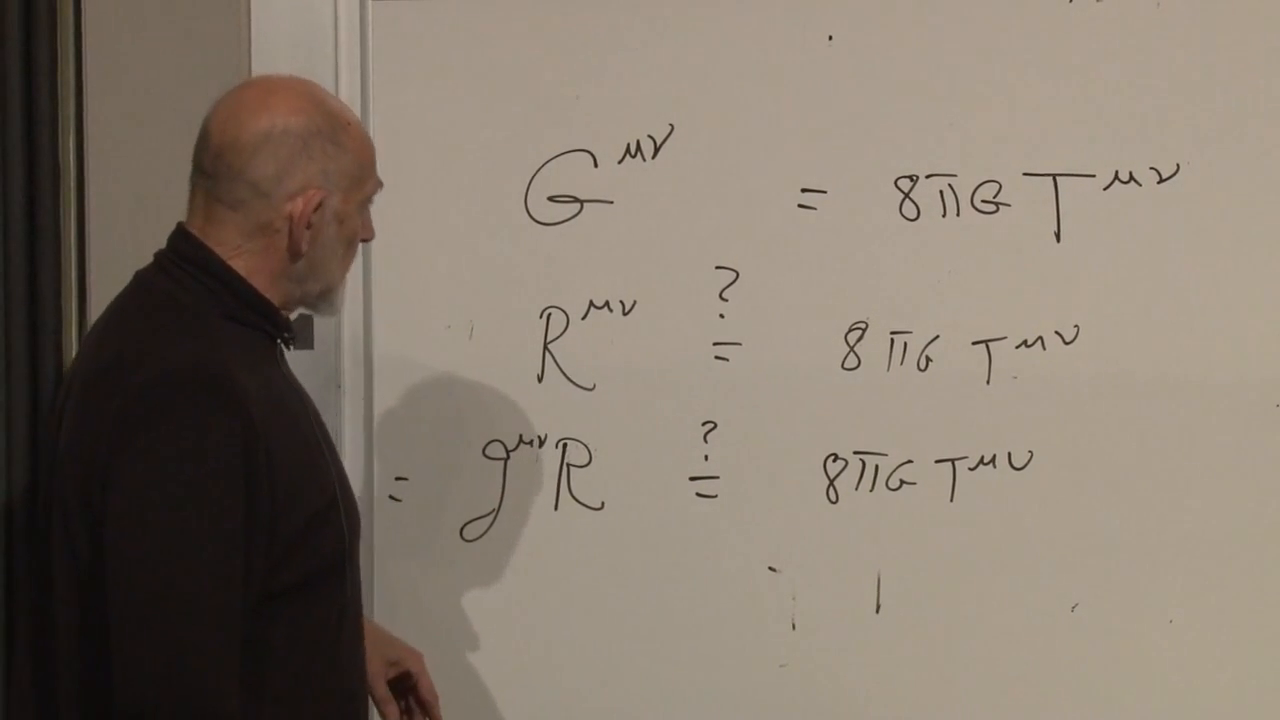
\includegraphics[width=0.78\textwidth]{lecture_09_figure_03.png}
\caption{Los dos tensores geométricos tentativos en la pizarra. En esta etapa ambos tienen el rango y el orden diferencial correctos, por lo que cada uno lleva un signo de interrogación.}
\lectureframe{01:04:56}
\end{figure}

Las alternativas exploratorias son
\begin{align}
 R_{\mu\nu}&\stackrel{?}{=}8\pi G\,T_{\mu\nu},\\
 g_{\mu\nu}R&\stackrel{?}{=}8\pi G\,T_{\mu\nu}.
\end{align}
No basta con aceptar ninguna de ellas porque sus índices encajen. La prueba es la conservación.

\section{La prueba de la divergencia}

Si la ecuación~\eqref{eq:field-schematic} es correcta, entonces debe cumplirse
\begin{equation}
 D_\mu G^{\mu\nu}=0
\end{equation}
porque \(D_\mu T^{\mu\nu}=0\). Empecemos por el candidato que contiene el escalar de curvatura. La regla del producto da
\begin{equation}
 D_\mu\!\left(g^{\mu\nu}R\right)
 =
 \left(D_\mu g^{\mu\nu}\right)R
 +g^{\mu\nu}D_\mu R.
 \label{eq:product-rule}
\end{equation}

\begin{figure}[htbp]
\centering
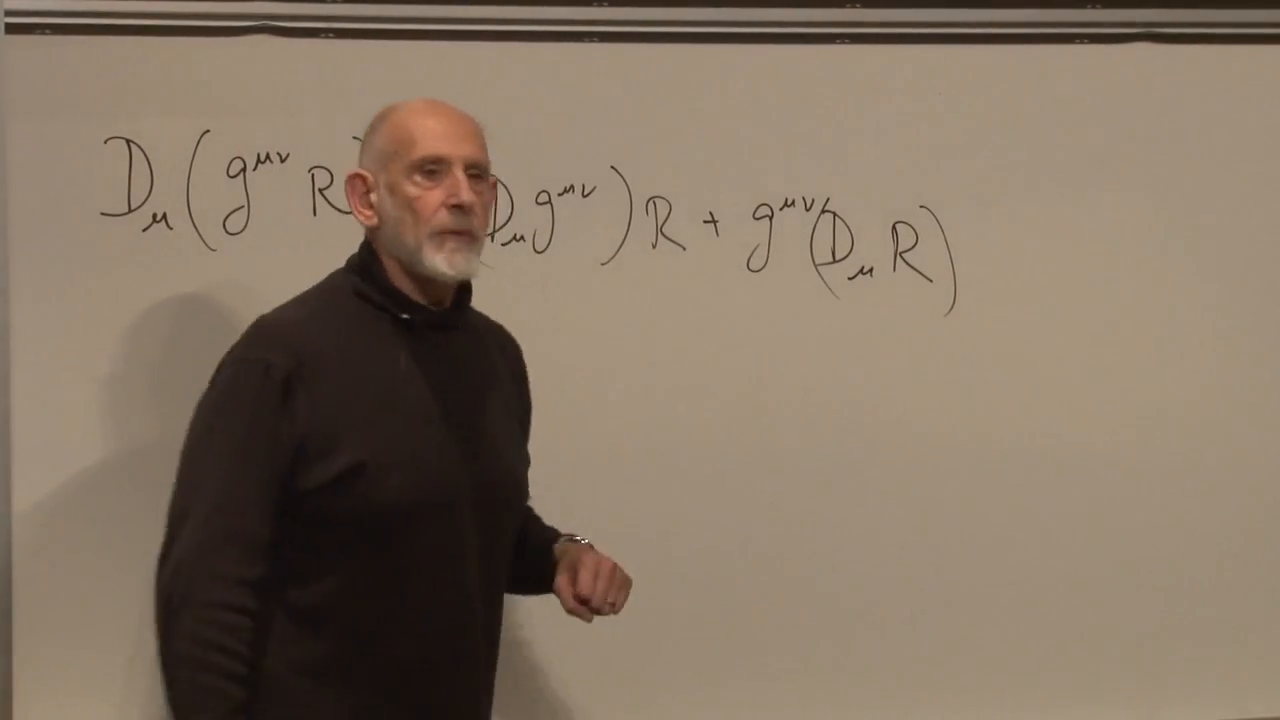
\includegraphics[width=0.84\textwidth]{lecture_09_figure_04.png}
\caption{Aplicación de la regla covariante del producto a \(D_\mu(g^{\mu\nu}R)\).}
\lectureframe{01:07:12}
\end{figure}

La compatibilidad métrica establece que
\begin{equation}
 D_\mu g^{\alpha\beta}=0.
 \label{eq:metric-compatibility}
\end{equation}
Esta es una propiedad geométrica independiente de la conexión de Levi-Civita, no una consecuencia de la conservación de energía-momento. Como \(R\) es un escalar, \(D_\mu R=\partial_\mu R\). Por tanto, la ecuación~\eqref{eq:product-rule} se convierte en
\begin{equation}
 D_\mu(g^{\mu\nu}R)
 =g^{\mu\nu}\partial_\mu R
 =D^\nu R,
\end{equation}
que, en general, no es cero. El candidato \(g^{\mu\nu}R\) falla.

El cálculo correspondiente para el tensor de Ricci es algo más largo. Su resultado es la identidad de Bianchi contraída,
\begin{equation}
 D_\mu R^{\mu\nu}=\frac12 D^\nu R.
 \label{eq:contracted-bianchi}
\end{equation}
Así, \(R^{\mu\nu}\) tampoco satisface por sí solo la condición. Pero los dos términos que fallan tienen exactamente la proporción necesaria para cancelarse:
\begin{equation}
 D_\mu\left(
 R^{\mu\nu}-\frac12 g^{\mu\nu}R
 \right)=0.
\end{equation}
Esto selecciona el tensor de Einstein,
\begin{equation}
 \boxed{
 G_{\mu\nu}
 =
 R_{\mu\nu}-\frac12 g_{\mu\nu}R
 }.
 \label{eq:einstein-tensor}
\end{equation}

Bajo los supuestos que usamos aquí--un tensor simétrico local de rango dos, construido a partir de la métrica y con no más de dos derivadas--esta combinación queda determinada salvo por un coeficiente global y un posible término proporcional a la métrica. Este último corresponde a la constante cosmológica, a la que volveremos hacia el final de la clase. El coeficiente que multiplica la ecuación~\eqref{eq:einstein-tensor} se fija al exigir que se recupere la gravedad newtoniana.

\begin{classroomqa}
\audiencequestion{¿Hay una manera más directamente física de obtener la ecuación de campo, en lugar de proponer candidatos y rechazarlos mediante la ecuación de continuidad?}
\lecturerresponse{La conservación local ya es un principio físico: la energía y el momento no pueden desaparecer de una región sin atravesar su frontera. También existe una derivación más condensada a partir de un principio de acción para el campo gravitatorio. Al variar esa acción se obtiene la misma ecuación, aunque el cálculo en sí no es breve.
\lecturetimestamp{01:17:14--01:18:41}}
\end{classroomqa}

\begin{classroomqa}
\audiencequestion{¿Podría algún otro tensor geométrico de rango dos satisfacer la misma ley de conservación? ¿La respuesta es física o matemática, y la habría conocido Einstein?}
\lecturerresponse{Bajo los supuestos de esta construcción, la clasificación es matemática. Los objetos de curvatura con dos derivadas disponibles se obtienen a partir del tensor de Riemann; los dos candidatos de rango dos que acabamos de examinar agotan las contracciones pertinentes. Encontrar la combinación cuya divergencia se anula sigue requiriendo un cálculo. Los principios son sencillos, pero manejar los índices y los signos es laborioso.
\lecturetimestamp{01:18:42--01:21:44}}
\end{classroomqa}

\section{La ecuación de campo y su límite newtoniano}

La ecuación de campo es ahora
\begin{equation}
 \boxed{
 R_{\mu\nu}-\frac12 g_{\mu\nu}R
 =
 8\pi G\,T_{\mu\nu}
 }.
 \label{eq:einstein-equation}
\end{equation}
El lado izquierdo es geométrico; el derecho describe la materia, la radiación y sus flujos. Las divergencias covariantes de ambos lados se anulan.

El factor \(8\pi G\) no se determina mediante el argumento de la divergencia. Se determina considerando un campo gravitatorio débil y de variación lenta, producido por materia que se mueve lentamente, y exigiendo que la componente temporal-temporal reproduzca la ecuación de Poisson. En ese régimen, \(T_{00}\simeq\rho\), mientras que las demás componentes están suprimidas por potencias de \(v/c\). El lado geométrico se reduce a la estructura de derivadas segundas anticipada en la ecuación~\eqref{eq:weak-mnemonic}. La comparación da exactamente la normalización de la ecuación~\eqref{eq:einstein-equation}.

Este límite también explica por qué parece que la gravedad newtoniana solo tiene como fuente la densidad de masa. En la teoría completa, gravita cada componente de \(T_{\mu\nu}\): la densidad de energía, el flujo de energía, la densidad de momento, la presión y el esfuerzo cortante. Para la materia ordinaria no relativista, domina la energía en reposo. En la materia relativista, la radiación o los sistemas con presiones elevadas, no se pueden ignorar las demás componentes.

La vía histórica no consistió en una única conjetura fácil. El tensor de Ricci parece el primer intento obvio, y el término adicional \(-\tfrac12g_{\mu\nu}R\) es lo que restablece la compatibilidad con la conservación local. Una vez fijada la estructura tensorial, el límite newtoniano determina la normalización.

\section{Lo que deja fuera una contracción}

\begin{classroomqa}
\audiencequestion{Cuando se contraen los cuatro índices del tensor de Riemann para reducirlos a dos, ¿tiene contenido físico la información descartada?}
\lecturerresponse{Sí. El tensor de Ricci no contiene toda la curvatura del espacio-tiempo. Los campos gravitatorios sin fuentes ofrecen los ejemplos más claros: el tensor de Ricci puede anularse mientras persisten la curvatura de marea y las ondas gravitatorias. La contracción conserva la parte vinculada directamente a la ecuación de la fuente local, pero no todos los grados de libertad del campo gravitatorio.
\lecturetimestamp{01:21:57--01:23:10}}
\end{classroomqa}

La analogía con el electromagnetismo resulta útil. Las ecuaciones de Maxwell admiten ondas en una región sin carga ni corriente. Del mismo modo, la ecuación de Einstein admite una geometría no trivial en una región donde \(T_{\mu\nu}=0\). Ahora derivaremos la ecuación más sencilla que se cumple allí.

\section{Vacío significa Ricci plano, no espacio-tiempo plano}

Tomemos
\begin{equation}
 T_{\mu\nu}=0.
\end{equation}
Entonces, la ecuación~\eqref{eq:einstein-equation} da
\begin{equation}
 R_{\mu\nu}-\frac12g_{\mu\nu}R=0.
 \label{eq:vacuum-einstein}
\end{equation}
Contraigamos con \(g^{\mu\nu}\). Como
\begin{equation}
 g^{\mu\nu}g_{\mu\nu}
 =\delta^\mu{}_\mu=4
\end{equation}
en cuatro dimensiones del espacio-tiempo, la traza es
\begin{equation}
 R-\frac12(4)R=-R=0.
\end{equation}
Por tanto,
\begin{equation}
 R=0,
 \qquad
 R_{\mu\nu}=0.
 \label{eq:ricci-flat}
\end{equation}
La ecuación de campo en el vacío es la condición de Ricci plano.

Es esencial no sustituir la expresión \emph{Ricci plano} por \emph{plano}.
El exterior de Schwarzschild no contiene materia fuera de la singularidad central y satisface \(R_{\mu\nu}=0\). Sin embargo, su tensor de Riemann es distinto de cero y las fuerzas de marea son reales. Se puede verificar que el espacio es Ricci plano calculando a mano todos los símbolos de Christoffel y las componentes de curvatura, aunque el cálculo es engorroso, o delegando esas operaciones a un sistema de álgebra simbólica. En la singularidad, las expresiones clásicas divergen; en todas partes fuera de ella se cumple la ecuación del vacío.

Las ondas gravitatorias son un segundo ejemplo. Pueden propagarse por una región sin fuentes y, a la vez, transportar una deformación real del espacio-tiempo. Así pues,
\begin{equation}
 R_{\mu\nu}=0
 \quad\not\Rightarrow\quad
 R^\rho{}_{\sigma\mu\nu}=0.
\end{equation}

\section{Conservar la fuente: la ecuación de la traza}

La clase casi termina con el resultado para el vacío, pero un asistente pide que se repita la contracción sin descartar la fuente.

\begin{classroomqa}
\audiencequestion{¿Qué se obtiene al hacer la misma contracción dejando \(T_{\mu\nu}\) en la ecuación?}
\lecturerresponse{La traza relaciona directamente el escalar de curvatura con la traza del tensor de energía-momento. Al sustituir esa relación de nuevo en la ecuación se obtiene una forma equivalente de la ecuación de campo expresada mediante el tensor de Ricci.
\lecturetimestamp{01:29:28--01:32:20}}
\end{classroomqa}

Definamos
\begin{equation}
 T=g^{\mu\nu}T_{\mu\nu}.
\end{equation}
Al tomar la traza de la ecuación~\eqref{eq:einstein-equation}, se obtiene
\begin{align}
 R-\frac12(4)R&=8\pi G\,T,\\
 -R&=8\pi G\,T,
\end{align}
por lo que
\begin{equation}
 \boxed{R=-8\pi G\,T}.
 \label{eq:trace-relation}
\end{equation}
Al sustituir de nuevo en la ecuación de campo, resulta
\begin{equation}
 \boxed{
 R_{\mu\nu}
 =
 8\pi G
 \left(
 T_{\mu\nu}-\frac12g_{\mu\nu}T
 \right)
 }.
 \label{eq:ricci-form}
\end{equation}

\begin{figure}[htbp]
\centering
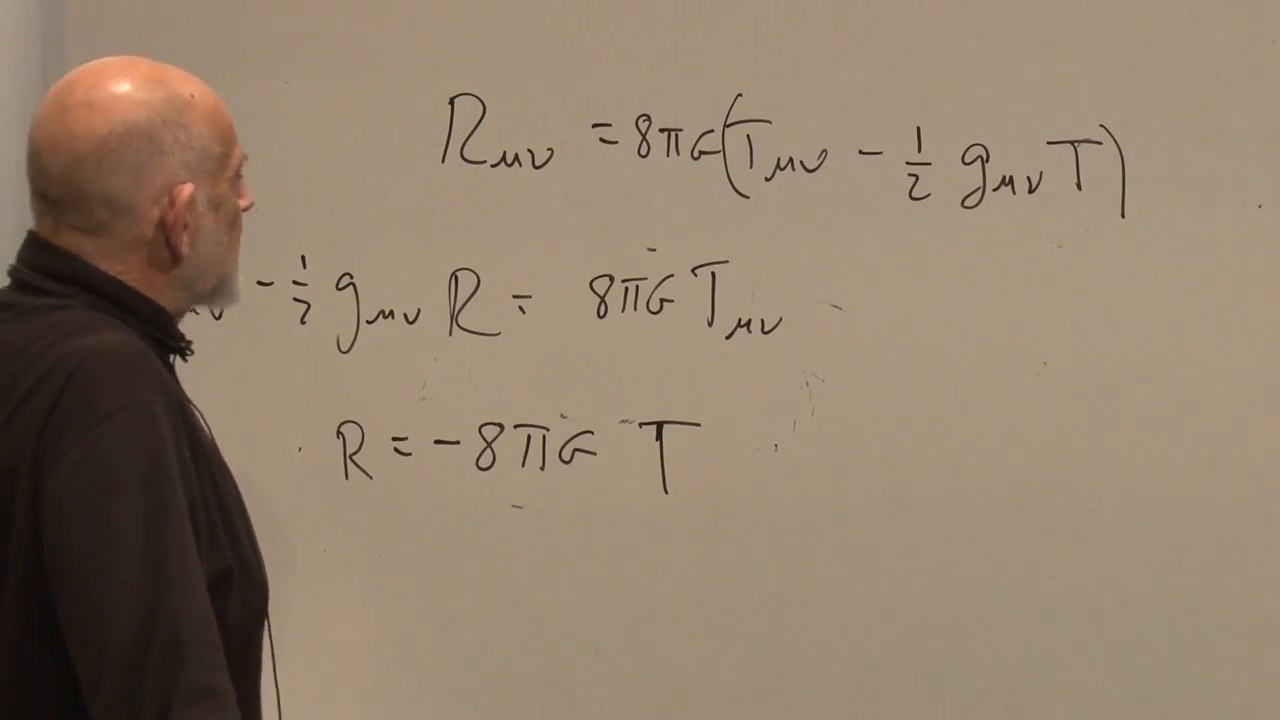
\includegraphics[width=0.82\textwidth]{lecture_09_figure_05.png}
\caption{La relación de la traza y la forma equivalente de la ecuación de Einstein expresada mediante el tensor de Ricci.}
\lectureframe{01:32:25}
\end{figure}

\begin{classroomqa}
\audiencequestion{¿Tiene significado físico el escalar \(T\)?}
\lecturerresponse{Es la traza del tensor de energía-momento. Para la radiación electromagnética es nula, y lo mismo ocurre con un gas ideal de partículas sin masa, como los fotones. La materia con masa suele tener una traza distinta de cero. Mediante la ecuación~\eqref{eq:trace-relation}, esa traza determina el escalar de curvatura.
\lecturetimestamp{01:32:20--01:33:12}}
\end{classroomqa}

\section{¿Cuánta curvatura recuerda Ricci?}

\begin{classroomqa}
\audiencequestion{¿Hay una imagen geométrica o física sencilla del tensor de Ricci y del escalar de Ricci, comparable al transporte paralelo alrededor de un lazo pequeño para el tensor de Riemann?}
\lecturerresponse{Aquí no se ofrece una imagen igual de transparente. El tensor de Riemann registra directamente la rotación producida al transportar un vector alrededor de un lazo pequeño. Sus contracciones son algebraicamente más sencillas, pero sus significados geométricos particulares son más difíciles de visualizar. Es mejor no inventar una imagen engañosa solo porque resultaría conveniente.
\lecturetimestamp{01:33:14--01:34:13}}
\end{classroomqa}

La cantidad de información que se pierde al contraer depende de la dimensión. En cuatro dimensiones, el tensor de Riemann contiene información sobre la curvatura que no está presente en el tensor de Ricci. En tres dimensiones, el tensor de Ricci determina el tensor de Riemann. En dos dimensiones, el escalar de curvatura contiene toda la información independiente sobre la curvatura. Por tanto, la gravedad en cuatro dimensiones admite grados de libertad de curvatura sin fuentes que \(R_{\mu\nu}\) no detecta.

\begin{classroomqa}
\audiencequestion{Si distintos tensores de Riemann pueden tener el mismo tensor de Ricci, ¿cómo se manifiesta físicamente la información que falta?}
\lecturerresponse{Una fuente dada no determina por sí sola todas las configuraciones gravitatorias posibles. Los datos de contorno y las condiciones iniciales pueden incluir radiación gravitatoria. En la aproximación de campo débil, se puede imaginar que se parte de una solución con fuente y se le añade una onda gravitatoria libre. La teoría no lineal completa no permite una superposición arbitraria, pero el ejemplo identifica correctamente la información que falta: curvatura propagante que no queda determinada localmente por \(T_{\mu\nu}\).
\lecturetimestamp{01:37:05--01:38:59}}
\end{classroomqa}

Ahora encajan dos ejemplos de vacío. La geometría de Schwarzschild presenta curvatura de marea en el exterior de una masa. Una onda gravitatoria transporta curvatura que se propaga libremente. Ambas pueden satisfacer \(R_{\mu\nu}=0\) y seguir siendo no planas.

\section{La constante cosmológica}

\begin{classroomqa}
\audiencequestion{¿No existe ningún factor de ajuste adicional, como una constante cosmológica?}
\lecturerresponse{Se permite una constante cosmológica. Puede escribirse en el lado geométrico como una constante multiplicada por \(g_{\mu\nu}\), o trasladarse al lado derecho e interpretarse como una contribución del vacío al tensor de energía-momento. Son dos descripciones de la misma ecuación con una contabilidad distinta.
\lecturetimestamp{01:39:01--01:40:44}}
\end{classroomqa}

Con una constante cosmológica, una convención habitual es
\begin{equation}
 G_{\mu\nu}+\Lambda g_{\mu\nu}
 =
 8\pi G\,T_{\mu\nu}.
\end{equation}
Al trasladar el término adicional al lado derecho se define un tensor de esfuerzos efectivo del vacío,
\begin{equation}
 T_{\mu\nu}^{(\Lambda)}
 =
 -\frac{\Lambda}{8\pi G}g_{\mu\nu}.
\end{equation}
Como la compatibilidad métrica da \(D_\mu g^{\mu\nu}=0\), el término adicional satisface automáticamente la ley de conservación. Este es el término proporcional a la métrica que quedó abierto en el enunciado anterior de unicidad.

\section{Mercurio y el cálculo de campo débil}

\begin{classroomqa}
\audiencequestion{¿Usó Einstein esta ecuación para calcular la órbita de Mercurio? ¿Dónde se puede ver cómo hizo ese cálculo?}
\lecturerresponse{Einstein trabajó antes de que Schwarzschild proporcionara la solución exacta, así que utilizó una aproximación suficientemente precisa del campo exterior del Sol a grandes distancias. El radio del Sol y la órbita de Mercurio son enormes en comparación con el radio de Schwarzschild solar, por lo que las correcciones relativistas son pequeñas. Podía partir de una órbita kepleriana y calcular perturbativamente la corrección. Poco después, Schwarzschild obtuvo la solución exterior exacta, lo que permitió sistematizar el mismo cálculo.
\lecturetimestamp{01:40:46--01:43:48}}
\end{classroomqa}

La teoría de perturbaciones consiste precisamente en esto: partir de un problema ya resuelto y calcular el efecto de una pequeña corrección. La fuerza newtoniana inversamente proporcional al cuadrado produce elipses keplerianas cerradas. La relatividad general añade una pequeña desviación a la ecuación radial newtoniana, por lo que la elipse no se cierra tras una revolución; su perihelio avanza.

La lección concluye con la curiosa singularidad de las órbitas bajo una fuerza central que se cierran. La fuerza inversamente proporcional al cuadrado de la distancia es excepcional porque hace que las órbitas keplerianas se cierren sin precesión. En términos más generales, el teorema de Bertrand identifica también al oscilador armónico isotrópico como el otro potencial central para el que toda órbita ligada se cierra. La pequeña corrección relativista elimina esa degeneración newtoniana y convierte la precesión de Mercurio en una señal observable de la ecuación de campo deducida en este capítulo.